% Chapter Template

\chapter{Background} % Main chapter title

\label{Chapter3} % Change X to a consecutive number; for referencing this chapter elsewhere, use \ref{ChapterX}

%----------------------------------------------------------------------------------------
%	SECTION 1
%----------------------------------------------------------------------------------------

\section{SMA (ou Système Multi-agent)}

En informatique, un système multi-agent (SMA) est un système composé d'un ensemble d'agents (un processus, un robot, un être humain, etc.), situés dans un certain environnement et interagissant selon certaines relations. Un agent est une entité caractérisée par le fait qu'elle est, au moins partiellement, autonome.
Objet de longue date de recherches en intelligence artificielle distribuée, les systèmes multi-agents forment un type intéressant de modélisation de sociétés, et ont à ce titre des champs d'applications larges, allant des sciences humaines, jusqu’aux services militaires et médicaux. \parencite{sma}


%-----------------------------------
%	SUBSECTION 1
%-----------------------------------
\subsection{Exemple de SMA de jeu vidéo}

Les communautés virtuelles que l’on trouve de plus en plus dans les jeux vidéo sont un parfait exemple afin de mieux comprendre le fonctionnement d’un SMA, par exemple, un jeu qui simulerait la vie d’une famille, plusieurs dimensions composent alors ce SMA.

~\par
Premièrement, un environnement ayant comme paramètre sa taille qui pourrait se caractériser par la maison et son jardin. Deuxièmement, les agents de ce SMA disposent d’une quantité d’objets dits “passifs” avec lesquels ils peuvent interagir, ce sera l’équipement de la maison ou encore la nourriture. Ensuite, les agents eux-mêmes, actifs et autonomes, ils sont en contact avec tout ce qui les entoure, leurs environnements, les objets qui le composent ou encore les autres agents, on les identifie comme étant “les membres de la famille”. On intègre ensuite le concept d’organisation, constitué des différentes relations entre les objets et les agents, liens familiaux, notions de propriété(qui possède tel ou tel objet). Pour finir, on ajoute des opérateurs qui permettent aux agents d’agir sur leur environnement ou sur les autres agents (le fils peut manger un yaourt, promener son chien ou parler à sa sœur)
Enfin, on intègre un ensemble d'opérateurs qui permettent aux agents d'agir sur les objets ou sur les autres agents (le fils peut promener son chien ou manger un yaourt ou parler à son père), et de capteurs qui permettent aux agents de connaître les changements de l'environnement et des autres agents (le yaourt est tombé par terre, papa m'a demandé de sortir le chien). Voici donc ce que l'on peut appeler un SMA. \parencite{sma}


\subsection{Exemple de SMA en opération “SWARMM” (Smart Whole Air Mission Model)} \label{ssec:swarm}

le  programme “SWARMM” a été développé par la division des opérations aériennes de l’organisation australienne de défense de science et technologies, il a  pour objectif de simuler les opérations des avions de combat pour la flotte aérienne australienne “La Royal Australian Air Force”.

~\par
Chaque pilote est un agent programmé avec dMARS, un environnement de programmation basé sur BDI(Belief-desire-intention ou Croyance-désir-intention) implémenté en FORTRAN et en C, chacun d'entre eux recevant des données des modèles physiques équivalents à ceux qu'un pilote reçoit de sa vision et de ses instruments et effectuant ce qui suit:

~\par
\begin{itemize}
\item Cycle de prise de conscience de la situation lorsque les données sont plus complexes (descripteurs symboliques)
\item  Évaluation de la situation, la situation est basée sur les résultats précédents de l'étape précédente.
\item Sélection tactique, sélectionnée en fonction de l'ensemble actuel d'objectifs qui a été reconnu lors des étapes précédentes
\item Procédures d'opération: choisies pour mettre en œuvre une tactique.
\end{itemize}

~\par
Plus d'une décennie de contacts étroits, d'entretiens avec des combattants, de briefing de missions et d'implication dans des exercices d'entraînement a été nécessaire afin d’arriver à établir ce cycle, il s’est avéré être d’une très grande valeur car il permet une intégration simple des procédures standard et de manière très documentée, il permet aussi aux combattants de décrire facilement leurs connaissances en se basant sur les différentes étapes du cycle et pour finir, il assure un échange simple compris entre les deux partis, pilotes et programmeurs, les programmeurs peuvent ainsi décrire leur résultat et débattre avec les pilotes en utilisant des termes similaires, il est principalement  basé sur le travail d’équipe et s’est avéré être extrêmement utile pour tester de nouveaux équipements et tactiques.

~\par
L’un des principaux buts du projet était  l’introduction d’un pilote (agent humain) dans la boucle de simulation en tant que coéquipier ou adversaire, il a donc été prouvé que même si pour un observateur extérieur ce programme ressemble à un vrai pilote, il n’était pas crédible aux yeux des vrais pilotes, et cela aux vues de son comportement extrêmement rationnel et peu naturel. \parencite{norling2000enhancing}


\section{NDM ( Naturalistic Decision Making)}

\begin{quotation}
“ L’étude de la NDM  pose la question de comment des individus expérimentés, travaillant individuellement ou en groupes, dans un environnement dynamique, rapide et incertain, identifient et évaluent leurs situations, prennent des décisions et effectuent des actions qui ont des conséquences signifiantes sur eux ainsi que sur l'organisation dans laquelle ils opèrent ” \parencite{zsambok2014naturalistic} \end{quotation} 



Ce terme est apparu en 1989 lors d’ateliers de chercheurs qui avaient pour but d’étudier 
“les prises de décisions dans des contextes réalistes” (médecine, centrales nucléaires, planification exécutive), leurs études ont montrés que les théories classiques sur les prises de décisions n’étaient tout simplement pas applicables dans le monde réel, ils ont aussi prouvé que même lorsque les agents étaient entraînés à faire des choix rationnels, ces derniers ne le faisaient que rarement.

~\par
Il en a ainsi émergé une meilleure compréhension sur la manière dont nous procédons pour prendre des décisions dans des situations complexes, dans certains cas, nous procédons effectivement de manière rationnelle, où, une multitude d’options sont générées, et la “meilleure” est sélectionnée, mais il existe d’autres stratégies qui sont plus communément utilisées.

~\par
La recherche dans ce domaine est principalement destinée à la conception d’aides à la décision, mais ces résultats peuvent également être utilisés pour développer de meilleurs modèles cognitifs pour les humains lors des simulations.

~\par
Orasanu et Connolly \parencite{orasanu1993reinvention} énumèrent huit facteurs qui caractérisent les paramètres de prises de décisions en milieu naturel. De nombreuses études de prise de décision classiques ignorent ou limitent délibérément ces facteurs, ce qui rend la théorie du choix rationnel plus facile à appliquer.

~\par

Ces facteurs sont:
\begin{itemize}
\item Problèmes mal structurés.
\item Environnements dynamiques incertains.
\item Objectifs changeants, mal définis ou concurrents.
\item Boucles d'action / de rétroaction.
\item Le stress dû au temps.
\item Des enjeux trop élevés.
\item Plusieurs joueurs.
\item Objectifs organisationnels et normes.
\end{itemize}

~\par
Tous les facteurs ne sont pas présents dans un contexte dit “naturel”, mais chacun ajoute une complexité au problème.


\subsection{Modèles de NDM}

Plusieurs modèles de prise de décision naturaliste ont été proposés, mais à ce jour,
aucun d’entre eux ne rend compte du spectre complet des décisions pouvant être prises dans un contexte naturel. Lipshitz \parencite{lipshitz1993converging} donne un résumé de neuf modèles qu’il souligne entre non contradictoires, mais illustrent les différents types de prise de décision qui peuvent être utilisés.

~\par
Notez que les chercheurs dans ce domaine s'intéressent généralement aux personnes qui sont expérimentées dans leur domaine. Hubert Dreyfus explique «le modèle d’acquisition de compétences en cinq étapes dans \parencite{dreyfus2014intuitive}, avec des niveaux allant de novice (quelqu'un qui débute dans  le domaine, comme un apprenti pilote), à un expert (quelqu'un qui est très habile et immergé dans son activité). La plupart des modèles NDM supposent un certain niveau d'expertise dans le domaine, pas nécessairement expert, mais certainement pas novice. L’un des modèles les plus connus est celui de Klein intitulé  “recognition-primed decision making” Modèle (RPD),  ou “la prise de décision axée sur la reconnaissance”. \parencite{klein2017sources}, illustré à la Figure \ref{fig:klein}.

~\par
Comme le souligne Klein lui-même «Le modèle RPD n'est pas issue de recherches en NDM »(\parencite{klein2017sources}, p.102), mais des études d’experts dans divers domaines montrent qu’une grande partie de leurs décisions sont prises de cette façon (voir le tableau 7.2 dans \parencite{klein2017sources}). La chose importante à noter à propos de ce modèle est l'accent qui est mis sur l'évaluation de la situation. Une fois que le décideur a reconnu la situation, il existe quatre sous-produits:

\begin{enumerate}

\item Il / elle s'attend à ce que certaines choses se produisent mais pas d'autres.
\item Il / elle fait attention à certains signaux pour soutenir le diagnostic.
\item Il existe une certaine compréhension des objectifs qu'il est plausible de réaliser.
\item et certaines actions sont susceptibles de réussir.
\end{enumerate}

Le décideur choisit ensuite une action, exécute une rapide simulation mentale de
celle-ci, et s'il/elle pense que cela va réussir, la met en œuvre. Une fois que le plan d’action  a été sélectionné et qu’il est entamé, la situation est surveillée pour s’assurer qu’elle se déroule comme prévu, sinon, d’autres actions pourraient être envisagées, mis à part cette éventualité, le décideur n'envisage pas d'autres options. (Notez que cet aspect du modèle n’est pas indiqué dans le diagramme.) Dans le modèle RPD, un opérateur expérimenté
choisira généralement «automatiquement» un plan d’action une fois que la situation est
reconnue, et que ce plan d’action est susceptible d’être celui qui a donné  auparavant
des résultats positifs dans la même situation.


\begin{figure}[th]
\centering
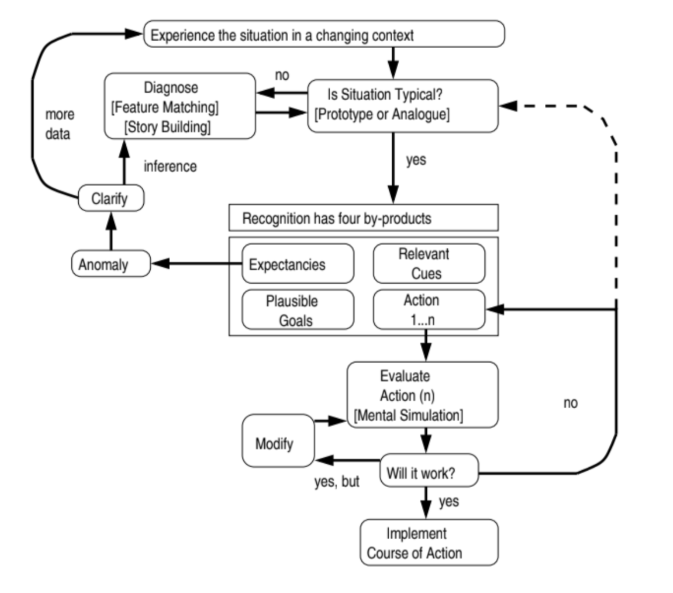
\includegraphics{Figures/klein.PNG}
\decoRule
\caption[ La version intégrée  du modèle de Klein de décision axée sur la reconnaissance] { La version intégrée  du modèle de Klein de décision axée sur la reconnaissance
(Figure 7.1 du livre “Sources of Power” by G. Klein 1998 \parencite{klein2017sources}) }
\label{fig:klein}
\end{figure}


~\par
Ce modèle [Figure \ref{fig:klein}, Page \pageref{fig:klein}] exprime l’idée qu’une personne qui acquiert de l’expertise est plus susceptible 
de reconnaître les subtilités entre les situations et de choisir un plan d’action en conséquence.



~\par

\section{Une brève histoire des jeux dans la recherche sur l'IA}

Les jeux ont une longue histoire dans la recherche sur l'IA, remontant au moins à 1949 lorsque Claude Shannon (peu après avoir développé l'entropie d'informations) s'est intéressé à l'écriture d'un programme informatique pour jouer au jeu d'échecs. Dans son article «Programmer un ordinateur pour jouer aux échecs», Shannon écrit:

~\par
“La machine à échecs est un système idéal pour commencer, car: 

~\par
\begin{enumerate}
\item Le problème est clairement défini à la fois dans les opérations autorisées (les mouvements) et dans le but ultime (le maté); 
\item Il n'est ni si simple d'être trivial ni trop difficile pour une solution satisfaisante; 
\item Les échecs sont généralement considérés comme nécessitant une «réflexion» pour un jeu habile; une solution de ce problème nous obligera soit à admettre la possibilité d'une pensée mécanisée, soit à restreindre davantage notre concept de «pensée»; 
\item La structure discrète des échecs s’intègre parfaitement dans la nature numérique des ordinateurs modernes.”

\end{enumerate}

C'était en 1949.

~\par
Depuis lors, il existe un intérêt durable pour la création de programmes informatiques capables de jouer à des jeux aussi habiles que des joueurs humains, même en battant les champions du monde respectifs. Shannon a inspiré le travail fondateur d’Arthur Samuel sur Checkers dans les années 1950 et 1960. Si le programme de Samuel n’a pas pu battre les experts, il a été considéré comme une réalisation majeure, car il s’agissait du premier programme à utiliser efficacement les procédures de recherche heuristique et les méthodes basées sur l’apprentissage. \parencite{unity1}


~\par
Chinook, un programme de contrôleurs mis au point à l’Université de l’Alberta en 1989, a commencé à battre les joueurs les plus humains et, dès 1994, les meilleurs joueurs pouvaient au mieux égaliser la machine. Cette tendance s’est poursuivie avec d’autres jeux de plateau à 2 joueurs tels que Backgammon (avec TD-Gammon de Gerald Tesauro, 1992-2002) et Chess (lorsque Deep Blue d’IBM a battu Garry Kasparov, 1997), et plus récemment avec Go.

~\par
Une avancée scientifique importante de ces dernières années a été celle où, en 2016, AlphaGo de DeepMind a battu le champion du monde 18 fois Lee Sedol 4 à 1, faisant l’objet du documentaire Netflix, AlphaGo. 


